
%(BEGIN_QUESTION)
% Copyright 2011, Tony R. Kuphaldt, released under the Creative Commons Attribution License (v 1.0)
% This means you may do almost anything with this work of mine, so long as you give me proper credit

This motor-control system uses a PLC to sequence the energization of two contactors: one ``low-speed'' contactor and one ``high-speed'' contactor.  The motor starts up on the low-speed contactor, then switches to the high-speed contactor after a few seconds in order to provide a more gentle start-up than a simple across-the-line starter arrangement.  All three-phase power conductors have been omitted from this illustration for simplicity:

$$\includegraphics[width=15.5cm]{i03506x01.eps}$$

Suppose a {\it short-circuit} develops in the coil of the high-speed contactor.  Explain what effect(s) this fault will have on the operation of the motor.

\underbar{file i03506}
%(END_QUESTION)





%(BEGIN_ANSWER)

Given a short-circuit fault in the coil of the high-speed contactor, the fuse will blow whenever the PLC tries to switch the motor to high-speed operation.  The motor will start up on low-speed, then the fuse will blow (and everything will power down) as soon as it tries to engage high-speed.

\vskip 10pt

Note: award only half-credit if the answer merely says something like ``the motor will only run in low speed'' and does not suggest the motor will stop running once the PLC attempts to engage high speed.

%(END_ANSWER)





%(BEGIN_NOTES)

{\bf This question is intended for exams only and not worksheets!}.

%(END_NOTES)

